\hypertarget{pf__search_8c}{
\section{pf\_\-search.c File Reference}
\label{pf__search_8c}\index{pf\_\-search.c@{pf\_\-search.c}}
}
{\tt \#include $<$stdio.h$>$}\par
{\tt \#include $<$stdlib.h$>$}\par
{\tt \#include $<$errno.h$>$}\par
{\tt \#include $<$string.h$>$}\par
{\tt \#include $<$sqlite3.h$>$}\par
{\tt \#include \char`\"{}libphonefirewall.h\char`\"{}}\par
{\tt \#include \char`\"{}logfile.h\char`\"{}}\par


Include dependency graph for pf\_\-search.c:\nopagebreak
\begin{figure}[H]
\begin{center}
\leavevmode
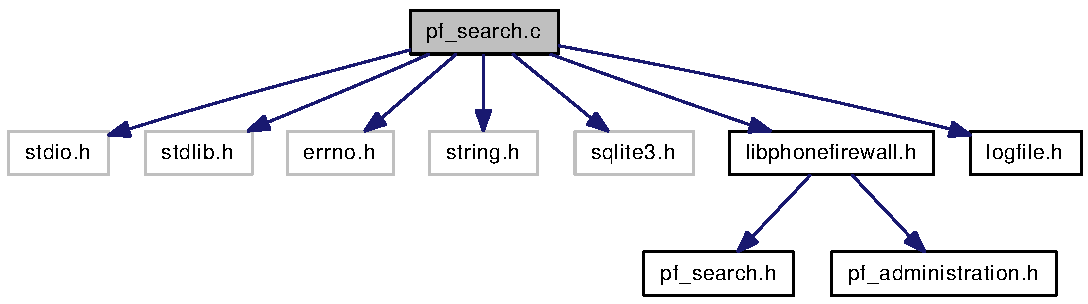
\includegraphics[width=279pt]{pf__search_8c__incl}
\end{center}
\end{figure}
\subsection*{Defines}
\begin{CompactItemize}
\item 
\#define \hyperlink{pf__search_8c_08df828ef9e922fa3a749f9bc0e4a42b}{ASCII\_\-PERCENT\_\-CHAR}~37
\item 
\#define \hyperlink{pf__search_8c_3b5bf1ced2c3343708fd193a487c2e26}{MAX\_\-ENTRY\_\-ARRAY}~1024
\end{CompactItemize}
\subsection*{Functions}
\begin{CompactItemize}
\item 
struct \hyperlink{structEntry}{Entry} $\ast$ \hyperlink{pf__search_8c_bc4a987c792bc712e4f1804a6f8be6b2}{find\_\-entry\_\-by\_\-name} (sqlite3\_\-stmt $\ast$pp\_\-stmt, char $\ast$name)
\item 
struct \hyperlink{structEntry}{Entry} $\ast$ \hyperlink{pf__search_8c_3947a1543660e9f6e666242efee44f89}{get\_\-entry\_\-by\_\-name} (char $\ast$name, int listflag)
\item 
struct \hyperlink{structEntry}{Entry} $\ast$ \hyperlink{pf__search_8c_678d356be18c20e298d74a62bc6e8782}{get\_\-entry\_\-by\_\-number} (int country\_\-code, int area\_\-code, unsigned long long number, int listflag)
\item 
struct \hyperlink{structEntry}{Entry} $\ast$ \hyperlink{pf__search_8c_b4e0af5dc1b0cf0bdd5812c973dcd353}{get\_\-entry\_\-by\_\-reason} (char $\ast$reason, int listflag)
\end{CompactItemize}
\subsection*{Variables}
\begin{CompactItemize}
\item 
struct \hyperlink{structEntry}{Entry} $\ast$ \hyperlink{pf__search_8c_6065da0f6097ff02236ecc4b7d04c912}{p\_\-entry} = \&\hyperlink{structentry}{entry}
\item 
struct \hyperlink{structEntry}{Entry} \hyperlink{pf__search_8c_4ac6231c71a3f59eeb4ae2462fb4dd54}{entry\_\-array} \mbox{[}MAX\_\-ENTRY\_\-ARRAY\mbox{]}
\end{CompactItemize}


\subsection{Define Documentation}
\hypertarget{pf__search_8c_08df828ef9e922fa3a749f9bc0e4a42b}{
\index{pf\_\-search.c@{pf\_\-search.c}!ASCII\_\-PERCENT\_\-CHAR@{ASCII\_\-PERCENT\_\-CHAR}}
\index{ASCII\_\-PERCENT\_\-CHAR@{ASCII\_\-PERCENT\_\-CHAR}!pf_search.c@{pf\_\-search.c}}
\subsubsection{\setlength{\rightskip}{0pt plus 5cm}\#define ASCII\_\-PERCENT\_\-CHAR~37}}
\label{pf__search_8c_08df828ef9e922fa3a749f9bc0e4a42b}




Definition at line 30 of file pf\_\-search.c.

Referenced by get\_\-entry\_\-by\_\-name().\hypertarget{pf__search_8c_3b5bf1ced2c3343708fd193a487c2e26}{
\index{pf\_\-search.c@{pf\_\-search.c}!MAX\_\-ENTRY\_\-ARRAY@{MAX\_\-ENTRY\_\-ARRAY}}
\index{MAX\_\-ENTRY\_\-ARRAY@{MAX\_\-ENTRY\_\-ARRAY}!pf_search.c@{pf\_\-search.c}}
\subsubsection{\setlength{\rightskip}{0pt plus 5cm}\#define MAX\_\-ENTRY\_\-ARRAY~1024}}
\label{pf__search_8c_3b5bf1ced2c3343708fd193a487c2e26}




Definition at line 31 of file pf\_\-search.c.

\subsection{Function Documentation}
\hypertarget{pf__search_8c_bc4a987c792bc712e4f1804a6f8be6b2}{
\index{pf\_\-search.c@{pf\_\-search.c}!find\_\-entry\_\-by\_\-name@{find\_\-entry\_\-by\_\-name}}
\index{find\_\-entry\_\-by\_\-name@{find\_\-entry\_\-by\_\-name}!pf_search.c@{pf\_\-search.c}}
\subsubsection{\setlength{\rightskip}{0pt plus 5cm}struct {\bf Entry}$\ast$ find\_\-entry\_\-by\_\-name (sqlite3\_\-stmt $\ast$ {\em pp\_\-stmt}, char $\ast$ {\em name})\hspace{0.3cm}{\tt  \mbox{[}read\mbox{]}}}}
\label{pf__search_8c_bc4a987c792bc712e4f1804a6f8be6b2}




Definition at line 36 of file pf\_\-search.c.

References Entry::area\_\-code, Entry::country\_\-code, Entry::name, Entry::number, Entry::priority, Entry::reason, TB\_\-AREACODE, TB\_\-COUNTRYCODE, TB\_\-NAME, TB\_\-NUMBER, TB\_\-PRIORITY, and TB\_\-REASON.

Referenced by get\_\-entry\_\-by\_\-name().

Here is the caller graph for this function:\nopagebreak
\begin{figure}[H]
\begin{center}
\leavevmode
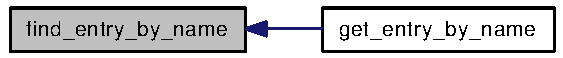
\includegraphics[width=153pt]{pf__search_8c_bc4a987c792bc712e4f1804a6f8be6b2_icgraph}
\end{center}
\end{figure}
\hypertarget{pf__search_8c_3947a1543660e9f6e666242efee44f89}{
\index{pf\_\-search.c@{pf\_\-search.c}!get\_\-entry\_\-by\_\-name@{get\_\-entry\_\-by\_\-name}}
\index{get\_\-entry\_\-by\_\-name@{get\_\-entry\_\-by\_\-name}!pf_search.c@{pf\_\-search.c}}
\subsubsection{\setlength{\rightskip}{0pt plus 5cm}struct {\bf Entry}$\ast$ get\_\-entry\_\-by\_\-name (char $\ast$ {\em name}, int {\em listflag})\hspace{0.3cm}{\tt  \mbox{[}read\mbox{]}}}}
\label{pf__search_8c_3947a1543660e9f6e666242efee44f89}


Search a \hyperlink{structentry}{entry} by name.

\begin{Desc}
\item[Parameters:]
\begin{description}
\item[{\em name}]The name of the person which is blocked. \item[{\em listflag}]A flag, which indicates if you would use the blacklist (BLACKLIST\_\-FLAG) or the whitelist (WHITELIST\_\-FLAG).\par
\end{description}
\end{Desc}
\begin{Desc}
\item[Returns:]\hyperlink{structentry}{entry} Returns the entries which are found in a linked list. \end{Desc}


Definition at line 67 of file pf\_\-search.c.

References Entry::area\_\-code, ASCII\_\-PERCENT\_\-CHAR, BLACKLIST\_\-FLAG, Entry::country\_\-code, DB\_\-FILE, entry\_\-array, ERR\_\-FLAG, find\_\-entry\_\-by\_\-name(), MAX\_\-LINE\_\-LENGTH, Entry::number, Entry::reason, STMT\_\-SIZE, TB\_\-AREACODE, TB\_\-COUNTRYCODE, TB\_\-NAME, TB\_\-NUMBER, TB\_\-PRIORITY, TB\_\-REASON, WHITELIST\_\-FLAG, and write\_\-logentry().

Here is the call graph for this function:\nopagebreak
\begin{figure}[H]
\begin{center}
\leavevmode
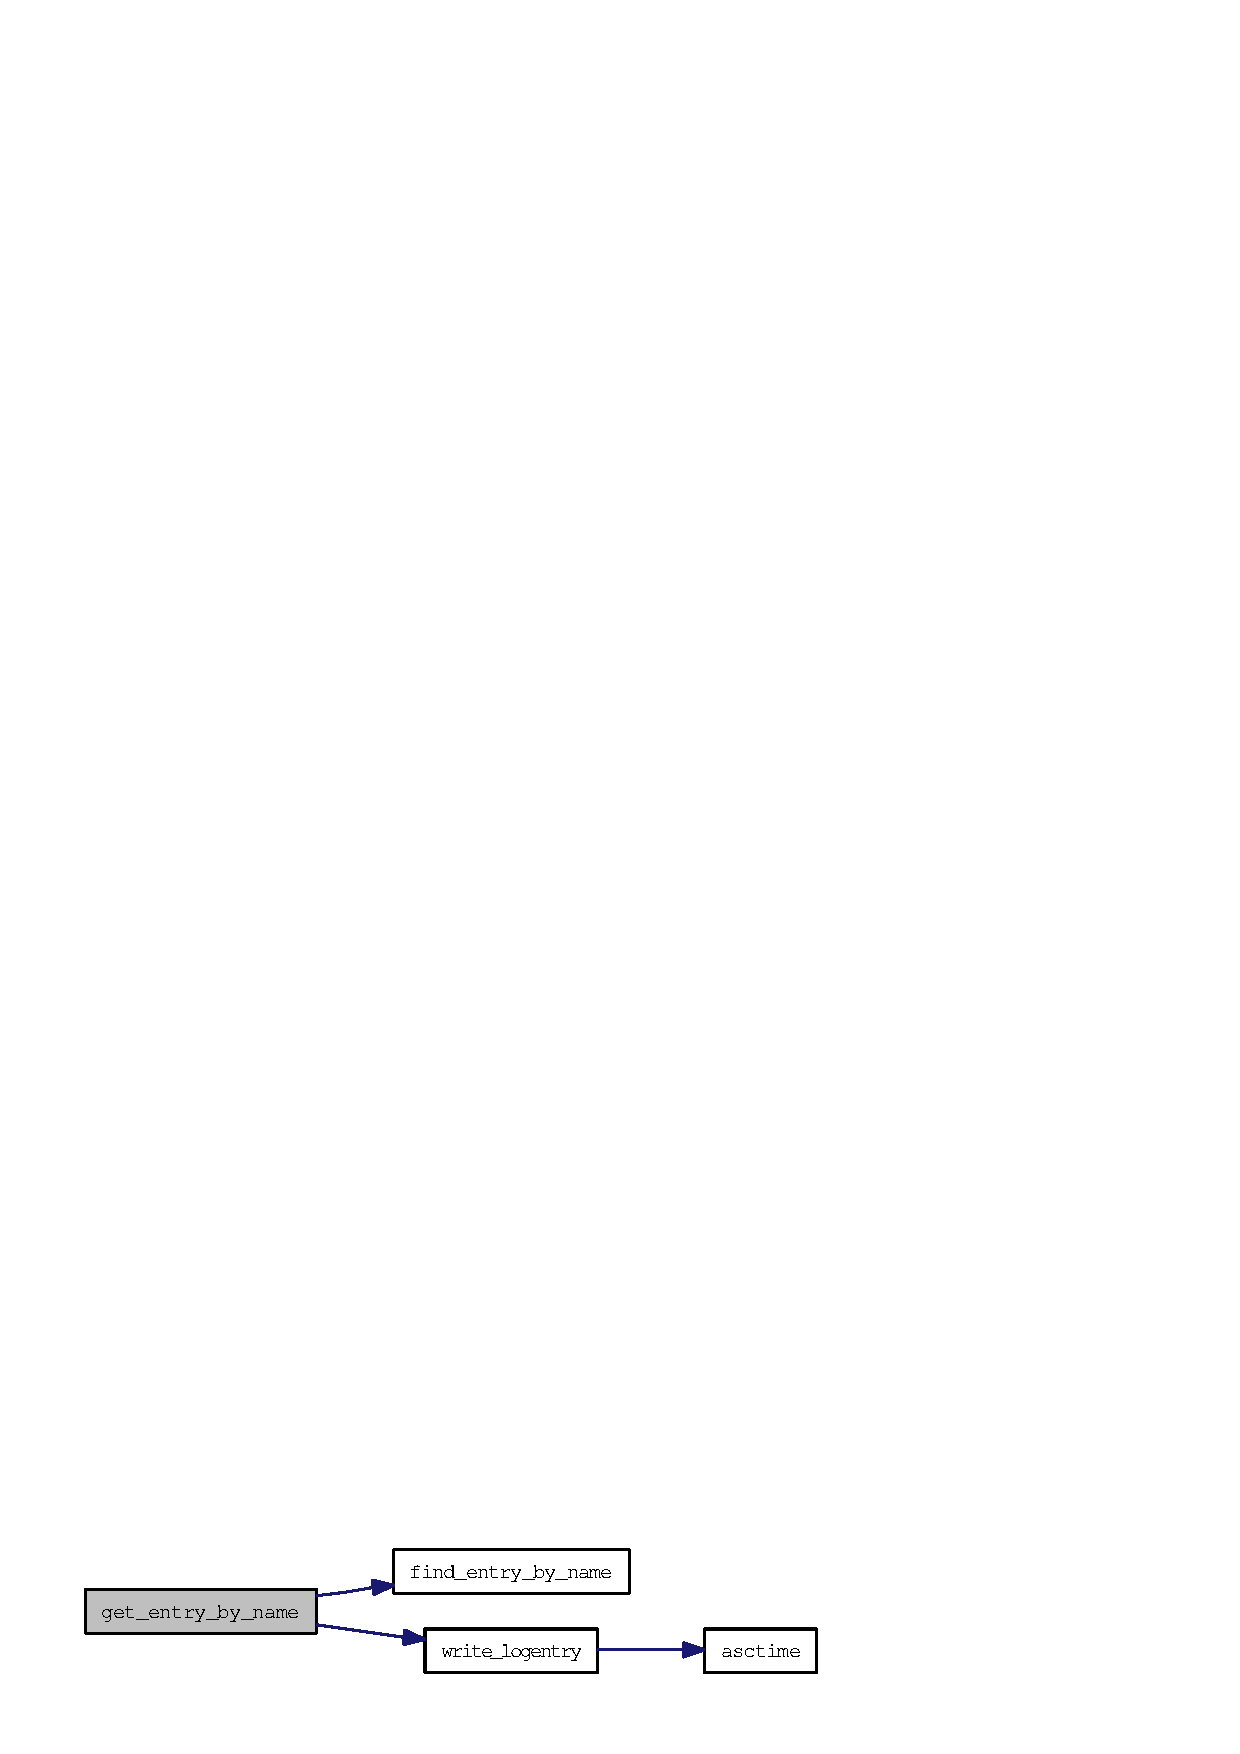
\includegraphics[width=198pt]{pf__search_8c_3947a1543660e9f6e666242efee44f89_cgraph}
\end{center}
\end{figure}
\hypertarget{pf__search_8c_678d356be18c20e298d74a62bc6e8782}{
\index{pf\_\-search.c@{pf\_\-search.c}!get\_\-entry\_\-by\_\-number@{get\_\-entry\_\-by\_\-number}}
\index{get\_\-entry\_\-by\_\-number@{get\_\-entry\_\-by\_\-number}!pf_search.c@{pf\_\-search.c}}
\subsubsection{\setlength{\rightskip}{0pt plus 5cm}struct {\bf Entry}$\ast$ get\_\-entry\_\-by\_\-number (int {\em country\_\-code}, int {\em area\_\-code}, unsigned long long {\em number}, int {\em listflag})\hspace{0.3cm}{\tt  \mbox{[}read\mbox{]}}}}
\label{pf__search_8c_678d356be18c20e298d74a62bc6e8782}


Search a entries by number (country code + area code + number).

\begin{Desc}
\item[Parameters:]
\begin{description}
\item[{\em country\_\-code}]The country code (for example 39 for Italy, 43 for Austria, and so one) \item[{\em area\_\-code}]The area code which indicates your mobile operator. \item[{\em number}]The telephone number of the person (without country and area code. \item[{\em listflag}]A flag, which indicates if you would use the blacklist (BLACKLIST\_\-FLAG) or the whitelist (WHITELIST\_\-FLAG).\par
\end{description}
\end{Desc}
\begin{Desc}
\item[Returns:]\hyperlink{structentry}{entry} Returns the entries which are found in a linked list. \end{Desc}


Definition at line 128 of file pf\_\-search.c.\hypertarget{pf__search_8c_b4e0af5dc1b0cf0bdd5812c973dcd353}{
\index{pf\_\-search.c@{pf\_\-search.c}!get\_\-entry\_\-by\_\-reason@{get\_\-entry\_\-by\_\-reason}}
\index{get\_\-entry\_\-by\_\-reason@{get\_\-entry\_\-by\_\-reason}!pf_search.c@{pf\_\-search.c}}
\subsubsection{\setlength{\rightskip}{0pt plus 5cm}struct {\bf Entry}$\ast$ get\_\-entry\_\-by\_\-reason (char $\ast$ {\em reason}, int {\em listflag})\hspace{0.3cm}{\tt  \mbox{[}read\mbox{]}}}}
\label{pf__search_8c_b4e0af5dc1b0cf0bdd5812c973dcd353}


Search a entries by reason.

\begin{Desc}
\item[Parameters:]
\begin{description}
\item[{\em reason}]The reason why a person is blocked/accpeted. \item[{\em listflag}]A flag, which indicates if you would use the blacklist (BLACKLIST\_\-FLAG) or the whitelist (WHITELIST\_\-FLAG).\par
\end{description}
\end{Desc}
\begin{Desc}
\item[Returns:]\hyperlink{structentry}{entry} Returns the entries which are found in a linked list. \end{Desc}


Definition at line 136 of file pf\_\-search.c.

\subsection{Variable Documentation}
\hypertarget{pf__search_8c_4ac6231c71a3f59eeb4ae2462fb4dd54}{
\index{pf\_\-search.c@{pf\_\-search.c}!entry\_\-array@{entry\_\-array}}
\index{entry\_\-array@{entry\_\-array}!pf_search.c@{pf\_\-search.c}}
\subsubsection{\setlength{\rightskip}{0pt plus 5cm}struct {\bf Entry} {\bf entry\_\-array}\mbox{[}MAX\_\-ENTRY\_\-ARRAY\mbox{]}}}
\label{pf__search_8c_4ac6231c71a3f59eeb4ae2462fb4dd54}




Definition at line 34 of file pf\_\-search.c.

Referenced by get\_\-entry\_\-by\_\-name().\hypertarget{pf__search_8c_6065da0f6097ff02236ecc4b7d04c912}{
\index{pf\_\-search.c@{pf\_\-search.c}!p\_\-entry@{p\_\-entry}}
\index{p\_\-entry@{p\_\-entry}!pf_search.c@{pf\_\-search.c}}
\subsubsection{\setlength{\rightskip}{0pt plus 5cm}struct {\bf Entry}$\ast$ {\bf p\_\-entry} = \&{\bf entry}}}
\label{pf__search_8c_6065da0f6097ff02236ecc4b7d04c912}




Definition at line 33 of file pf\_\-search.c.

Referenced by check\_\-entry().